%*****************************************
\chapter{Preliminares de Grafos}\label{ch:preliminaresGrafos}
%*****************************************

TODO : introducción del capítulo
La teoría necesaria para comprender las aplicaciones de ZKP con grafos es muy básica, los resultados de esta sección se pueden consultar en \citep{grafosyOD}.
% TODO añadir bibliografía si falta

\hfil

\section{Teoría de grafos}

\begin{definition}
	Un \textit{grafo} (simple no dirigido) es un par $(V,E)$ formado por un conjunto finito $V \neq \emptyset$, a cuyos elementos denominaremos \textit{vértices} o \textit{nodos}, y $E$, un conjunto de pares (no ordenados y formados por distintos vértices) de elementos de $V$, a los que llamaremos \textit{aristas}.
	
	A los nodos $v_1$ y $v_2$ que forman una arista $e = (v_1, v_2)$ se les llama \textit{extremos} de $e$.
\end{definition}


\begin{definition}[Conceptos]
	\hfil
	
	A dos nodos $v_1$ y $v_2$ que forman parte de una misma arista se les llama \textit{adyacentes}.
	
	Se llama \textit{orden} de un grafo a $\mid V \mid $.
	
	Se llama \textit{tamaño} de un grafo a $\mid E \mid $.
	
	Un grafo con $ \mid V \mid = 1$ (consecuentemente $\mid E \mid = 0$) se llama \textit{trivial}.
	
	Se dice que una arista es \textit{incidente} con un vértice $v$ cuando $v$ es uno de sus extremos.
\end{definition}



\begin{definition}
	Dos grafos $G_1 = (V_1, E_1)$ y $G_2 = (V_2, E_2)$ se dice que son \textit{isomorfos}, lo cual denotaremos como $G_1 \simeq G_2$, si existe una aplicación biyectiva $\tau : V_1 \rightarrow V_2$ tal que $\forall u,v \in V_1$
	
	\begin{center}
		$(u,v) \in E_1 \Leftrightarrow (\tau(u), \tau(v)) \in E_2 $.
	\end{center}
	
	Tal aplicación recibe el nombre de \textit{isomorfismo}. Si $G_1 = G_2$, llamaremos a $\tau$ \textit{automorfismo}.
\end{definition}

En un abuso de notación, podemos escribir que $\tau(G_1) = G_2$.


\hfil

Dados dos grafos $G_1 = (V, E_1)$ y $G_2 = (V, E_2)$ isomorfos, con el mismo conjunto de vértices, $V=\{v_1,\dots v_n\}$, vemos que el isomorfismo entre $G_1$ y $G_2$ puede denotarse como una permutación en el índice de sus nodos.

Utilizaremos la notación $Sym(V)$ para denotar los automorfismos de $G=(V,E)$, que será el grupo simétrico $S_n$ de las permutaciones de los vértices, cuando $\mid V \mid=n$. Por lo visto en los preliminares de álgebra, tenemos que $\mid Sym(V) \mid = n!$ .





\hfil


\paragraph{Coloración de grafos}
\hfil

\begin{definition}
	Una \textit{coloración} de un grafo $G=(V,E)$ es una aplicación $c:V\rightarrow \{1,2,\dots , l\}$.

	El valor $c(v_i)$ es el \textit{color} correspondiente al nodo $v_i$.
\end{definition}

\begin{definition}
	Una \textit{coloración propia} de un grafo es una coloración que hace corresponder colores diferentes a vértices adyacentes:

	$\forall (u,v)\in E \to c(u)\neq c(v)$.
\end{definition}


\begin{definition}
	Llamaremos \textit{número cromático} del grafo $G$, $\chi(G)$, al mínimo valor de $l$ que permite una coloración propia de $G$, es decir, al mínimo número de colores necesarios para colorear los vértices de forma que los extremos de cada arista tengan colores distintos.
\end{definition}


\begin{definition}
	Un \textit{grafo plano} es $(V,E)$, un par de conjuntos finitos llamados \textit{vértices} y \textit{aristas} que satisfacen:
	\begin{itemize}
		\item $V \subset \mathbb{R}^2$.
		\item Cada arista de $E$ es un arco entre dos vértices distintos.
		\item Aristas diferentes tienen extremos diferentes.
		\item El interior de una arista no contiene ni vértices ni puntos de otra arista.
	\end{itemize}

	Para cada grafo plano $G$, el conjunto $\mathbb{R}^2\setminus (V\cup E) $ es abierto. Sus regiones se llaman \textit{caras}.
\end{definition}

\begin{definition}
	Un grafo isomorfo a un grafo plano, se denomina \textit{grafo planar}.
	
	Cada representación de un grafo planar como un grafo plano se llama un \textit{embutido}.
\end{definition}

\begin{theorem}
	Si $G$ es un grafo planar, entonces $\chi(G) \leq 4$.
\end{theorem}

Este último resultado es el conocido como Teorema de los cuatro colores, que en una versión menos técnica dice:

\begin{theorem}
	Dado cualquier mapa geográfico con regiones continuas, este puede ser coloreado con cuatro colores diferentes, de forma que no queden regiones adyacentes con el mismo color.
\end{theorem}


\hfil




\paragraph{Caminos hamiltonianos}
\hfil


TODO

%%%%%%%%%%%%%%
%%%draft


\paragraph{Representación de grafos}
\hfil

%TODO: si no implementamos nada de grafos, no hace falta
\textbf{TODO: si no implementamos nada de grafos, no hace falta}

\hfil

Dado $G=(V,E)$ con $V=\{v_1,\dots v_n\}$ y $E=\{e_1,\dots e_m\}$, podemos representarla por:

\begin{itemize}
	\item  La \textit{matriz de adyacencia} $M_{nxn} = (m_{ij})$, que se construye mediante:
	\[
	m_{ij} =
	\begin{cases}
	1 & si\ (v_i,v_j) \in E \quad ( \Leftrightarrow (v_j,v_i)\in E ), \\
	0 & en\ otro\ caso.
	\end{cases}
	\]
	
	\item La \textit{matriz de incidencia} (vértice-arista) $M_{nxm} = (m_{ij})$ con
	\[
	m_{ij} =
	\begin{cases}
	1 & si\ v_i\ es\ extremo\ de\ e_j, \\
	0 & en\ otro\ caso.
	\end{cases}
	\]
	
	\item Una matriz de enteros $M_{mx2}$ cuyas filas contienen los índices de los extremos inicial y final de las aristas del grafo.
	
	\begin{example}
		El grafo:
		
		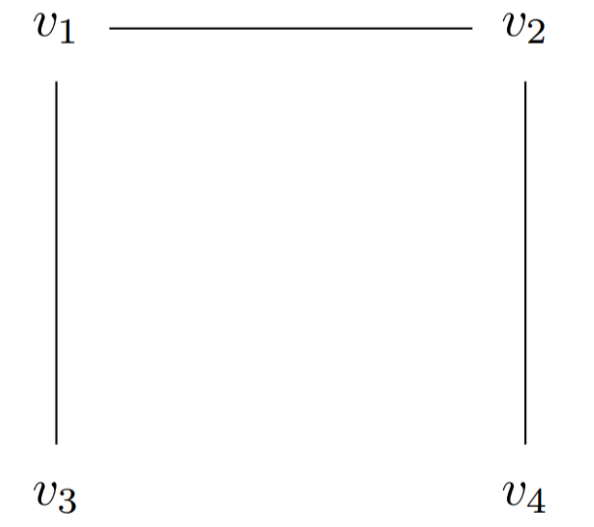
\includegraphics[width=.2\linewidth]{gfx/exgraph}
		\qquad se representaría como: \qquad
		\begin{tabular}{|c|c|}
			\hline	1 & 2 \\ \hline 1 & 3 \\ \hline 2 & 4 \\ \hline
		\end{tabular}	
		
	\end{example}
	
\end{itemize}



\section{Problemas de decisión basados en grafos}

A continuación, introducimos los enunciados de los problemas de grafos utilizados en pruebas de conocimiento cero, y referencias donde se estudian sus órdenes de complejidad.

\subsection{Problema del isomorfismo de grafos}

\hfil

\begin{tabular}{|ll}
	\textit{Nombre:} & Problema GI (\textit{Graph Isomorphism}). \\
	\textit{Parámetros:} & Dos grafos $G_0 = (V_0, E_0)$ y $G_1 = (V_1, E_1)$, \\ & del mismo orden $\mid V_0 \mid = \mid V_1 \mid = n$. \\
	\textit{Pregunta:} & ¿Existe un isomorfismo $\pi : V_0 \rightarrow V_1$ tal que \\ & una arista $(u,v)\in E_0$ si y solo si $(\pi (u),\pi (v)) \in E_1$? \\
\end{tabular}
\\

\hfil

%TODO
TODO

\subsection{Problema del camino hamiltoniano}

\hfil

\begin{tabular}{|ll}
	\textit{Nombre:} & Problema CH. \\
	\textit{Parámetros:} &Un grafo $G=(V,E)$. \\
	\textit{Pregunta:} & ¿Existe un ciclo en G que recorre pasa por\\& cada vértice en V una única vez? \\
\end{tabular}
\\

\hfil

TODO

\subsection{Problema de la 3-coloración}

\hfil

\begin{tabular}{|ll}
	\textit{Nombre:} & Problema G3C. \\
	\textit{Parámetros:} &Un grafo $G=(V,E)$. \\
	\textit{Pregunta:} & ¿Existe una función $\phi : V \to \{1,2,3\}$ tal que \\ & $\forall (u,v)\in E$, se cumple $\phi(u)\neq \phi(v)$? \\
\end{tabular}
\\

\hfil

TODO

